\chapter{Introduction}
\pagenumbering{arabic}
When we talk about communication we often mean the transfer or exchange of information between two subjects or groups. What sounds so simple takes on a new meaning when one understands how we managed to overcome immense distances to get closer together.

Since life evolved on Earth, communication has always been present. For example nerve cells use electrical or chemical synapses to communicate, animals communicate through a variety of different methods including pheromones and sounds and humans mainly communicate through the advantageous construct of language \cite{Christian:2004}.

Due to the limitation to communicate over long distances our ancestors invented different techniques to exchange information. One of the oldest known methods of such communication is that of smoke signals which were used to send messages in form of binary information. Much later, with the discovery of electricity, a new era for human communication began when Samuel Finley Breese Morse perfected line telegraphy in the 1830s \cite{Glover:2010}. Suddenly we were able to instantly exchange complex information over immense distances. From that point on, communication, or more precisely telecommunication, got more and more important and has developed rapidly in recent centuries. 

Nowadays telecommunication is an integral part of everyday life. A phone call connects us over several thousand kilometres, scientists can share their research through the vast network of the Internet globally and space probes, like NASA's Voyager 1 and Voyager 2, send us data and images from places, a few centuries ago, we never thought we could ever explore. 

For the future we can only dream. But with new knowledge, new technologies emerge.

\section{About the thesis}
This thesis about a voice communication system for a spacesuit simulator was not only proposed to design and build a working backup system for the Serenity spacesuit simulator of the Austrian Space Forum (OeWF), but also to continue humanity's ventures to explore the planet Mars and to add a tiny bit to the long history of telecommunication and space exploration. More about the OeWF and the Serenity spacesuit simulator can be found the appendix \ref{ap:oewf}.

\subsection{Motivation} 
The voice communication system described in this thesis is closely related to amateur radio systems. This brings an enormous advantage in the form of a solid market for components and the availability of knowledge from experienced amateur radio operators.

Over the years, amateur radios remained popular due to their reliability and independence from cellular networks and the Internet. Large communities enthusiastically take care of this independent infrastructure around the globe. But not only amateur radio operators use this infrastructure, emergency services such as the red cross, the police and fire departments as well as armed forces use professional radio equipment. It is therefore still considered a crucial infrastructure. 

This thinking can be applied to Serenity's backup voice communication system as well. The infrastructure that is used consists of commercially available equipment which can be procured, maintained, repaired and set up easily. Due to its close relation to amateur radio systems it can be used for local emergencies apart from the missions of the OeWF. In addition to these points, the repeater radio infrastructure of Serenity's backup voice communication system is designed to be completely self-sufficient which allows it to be operated in the field without an external power supply. This enables use in remote areas as well as on construction sites, for corporate communication, for disaster relief and for everyday communication by amateur radio operators.

\subsection{Backup voice communication system}
Analog astronauts rely on many critical subsystems, like the voice communication system, to keep them safe and protected while performing simulations. This system is so to speak the lifeline of the analog astronauts which helps them to keep in touch with each other, their safety officers and the base camp crew. For completeness it is noted that the safety officers are trained emergency first responders and the base camp crew monitors and coordinates analog Mars field  locally 

To guarantee flawless missions, a robust communication system is required. Therefore, the OeWF developed a primary voice communication system which is currently used in the Aouda spacesuit simulator. With several upgrades this system will be used in the Serenity spacesuit simulator as well. It is based on a \emph{wireless local area network} (WLAN) with a range of $15\mathrm{km}$ including a field infrastructure \cite{Groemer:2020}. Should this link fail, a dangerous situation for the analog astronauts can arise. In order to prevent such a situation, it is crucial to add redundancy in the form of a second, completely independent, voice communication system that serves as a backup. 

To keep up with the primary W-LAN based voice communication system, the OeWF decided to redesign and improve the backup voice communication system for the second generation of its spacesuit simulators. Serenity's backup voice communication system has to be more powerful and reliant than Aouda's. To achieve this goal, the OeWF came up with the requirements listed in the table \ref{tab:table_serenity_bu_comms_requirements}.
\begin{table}[h!]
	\centering
	\footnotesize
\begin{tabular}{|l|c|}
	\hline
	\multicolumn{2}{|c|}{\textbf{Requirements}} \\
 	\hline
 	Range (diameter of square) & $15\mathrm{km}$ \\
	Dimensions & Must fit inside the HUT. \\
	Operating temperature within the HUT & $5^\circ \mathrm{C}$ to $45^\circ \mathrm{C}$ \\
	Combined mass within the HUT & $1000\mathrm{g}$ \\
 	\hline
\end{tabular}
	\caption{Requirements for the voice communication systems of the Serenity spacesuit simulator.}
	\label{tab:table_serenity_bu_comms_requirements}
\end{table}

The backup voice communication system must cover at least a mission area that is created by a square with a diagonal of $15\mathrm{km}$. With regard to the Serenity spacesuit simulator, its designed backup radio system must fit into its \emph{hard upper torso} (HUT). Within the HUT it must function for the specified operating temperatures and the combined mass of the primary and backup radio systems must not exceed $1000\mathrm{g}$. 

\section{Aim}
The aim of this thesis is to design the backup voice communication system, which from now on will simply be referred to as voice communication system, for the Serenity spacesuit simulator and to carry out a performance estimation based on the design. This must be accomplished while taking into account the requirements mentioned in the table \ref{tab:table_serenity_bu_comms_requirements}. Since a repeater radio infrastructure for the voice communication system is necessary to meet the range requirement, a suitable self-sufficient energy distribution system is also designed alongside the voice communication system. A performance estimation is carried out for this system as well. In addition, it will be investigated how the designed voice communication system must be adapted so that it can be used on the Martian surface.

\subsection{Literature review}
Planning voice communication systems is explained in detail in various literatures. Depending on the application, different frequencies and directional characteristics of the antennas involved are used \cite{Lange:1992, Parsons:2000, Glover:2010, Goiser:2019, Mecklenbrauker:2017}. For voice communication, however, frequencies in the \emph{very high frequency} (VHF) and \emph{ultra high frequency} (UHF) bands are mostly used in combination with omnidirectional antennas, as the participants of the voice communication system usually move freely within a local covered area \cite{Parsons:2000}. Depending on the required planning accuracy, either a performance estimation is carried out with the plane earth signal budget, or with more complex caluculations that take the ground roughness, objects in the beam path between the transmitter and the receiver and atmopsheric effect into account \cite{Parsons:2000, Glover:2010, LinkMargin:2016, Mecklenbrauker:2017}.

There are also numerous books for planning energy distribution systems. The books \cite{Rebhan:2002, Gawlik:2018}, for example, provide an overview of how various forms of energy can be converted into electrical energy. Then works like \cite{Mertens:2015, Hau:2016, Wagner:2018} can be used to read into the energy conversion method that is ultimately used to supply a load with electrical energy. Apart from that, the works \cite{Sterner:2017, Kurzweil:2018} describe how the electrical energy can be stored if this is necessary. 

Regarding the planning of a voice communication and an energy distribution system on Mars, publications such as \cite{Appelbaum:1990, Appelbaum:1992, Landis:1995, Ho:2002} can be used. 

\subsection{Deliverables}
This subsection now summarizes the deliverables of the thesis.
\begin{enumerate}
  \item Design the backup voice communication system for the Serenity spacesuit simulator.
  \item Design a self-sufficient energy distribution system for the repeater radio infrastructure of the backup voice communication system.
  \item Provide a performance estimation of the voice communication system.
  \item Provide a performance estimation of the self-sufficient energy distribution system.
  \item Investigate the usability of the designed voice communication and energy distribution system on Mars.
\end{enumerate} 
The flowcharts in the figures \ref{fig:tikz_flowchart_1} and \ref{fig:tikz_flowchart_2}, illustrate which steps were taken to achieve these.
\begin{figure}[h!]
	\centering
	

\tikzset{every picture/.style={line width=0.75pt}} %set default line width to 0.75pt        

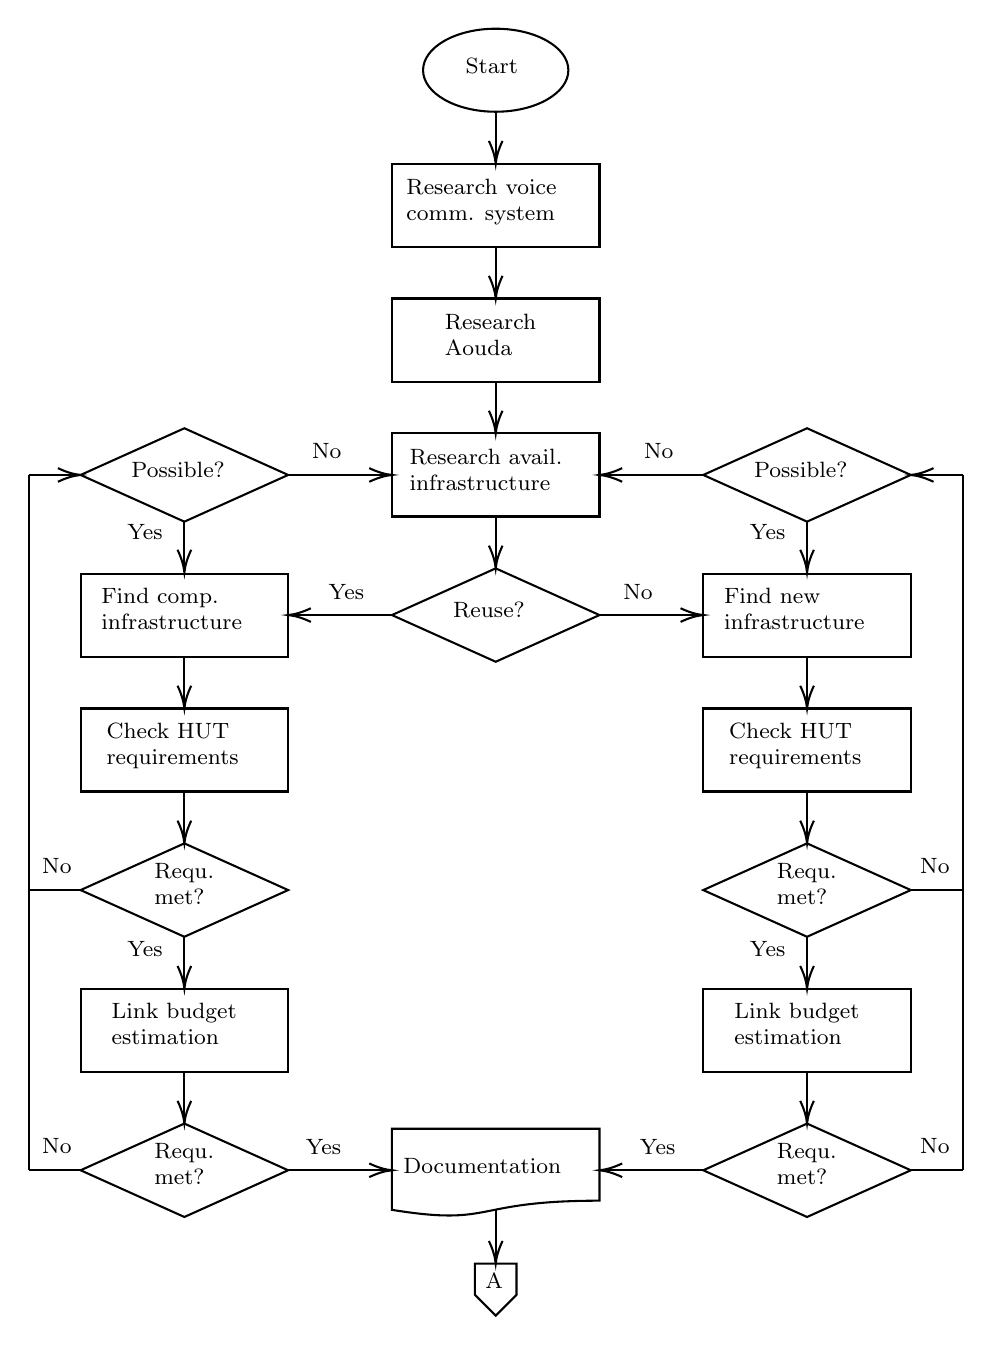
\begin{tikzpicture}[x=0.75pt,y=0.75pt,yscale=-1,xscale=1]
%uncomment if require: \path (0,667); %set diagram left start at 0, and has height of 667

%Shape: Diamond [id:dp04084543344377911] 
\draw   (145,202.5) -- (195,225) -- (145,247.5) -- (95,225) -- cycle ;
%Straight Lines [id:da3172337098532787] 
\draw    (243,225) -- (195,225) ;
\draw [shift={(245,225)}, rotate = 180] [color={rgb, 255:red, 0; green, 0; blue, 0 }  ][line width=0.75]    (10.93,-3.29) .. controls (6.95,-1.4) and (3.31,-0.3) .. (0,0) .. controls (3.31,0.3) and (6.95,1.4) .. (10.93,3.29)   ;

%Shape: Ellipse [id:dp5174120932429653] 
\draw   (260,30) .. controls (260,18.95) and (275.67,10) .. (295,10) .. controls (314.33,10) and (330,18.95) .. (330,30) .. controls (330,41.05) and (314.33,50) .. (295,50) .. controls (275.67,50) and (260,41.05) .. (260,30) -- cycle ;

%Straight Lines [id:da5375994326166968] 
\draw    (295,115) -- (295,138) ;
\draw [shift={(295,140)}, rotate = 270] [color={rgb, 255:red, 0; green, 0; blue, 0 }  ][line width=0.75]    (10.93,-3.29) .. controls (6.95,-1.4) and (3.31,-0.3) .. (0,0) .. controls (3.31,0.3) and (6.95,1.4) .. (10.93,3.29)   ;
%Shape: Rectangle [id:dp32571227246524637] 
\draw   (245,140) -- (345,140) -- (345,180) -- (245,180) -- cycle ;

%Straight Lines [id:da7335469832694597] 
\draw    (295,180) -- (295,203) ;
\draw [shift={(295,205)}, rotate = 270] [color={rgb, 255:red, 0; green, 0; blue, 0 }  ][line width=0.75]    (10.93,-3.29) .. controls (6.95,-1.4) and (3.31,-0.3) .. (0,0) .. controls (3.31,0.3) and (6.95,1.4) .. (10.93,3.29)   ;
%Shape: Rectangle [id:dp18134004375921853] 
\draw   (245,205) -- (345,205) -- (345,245) -- (245,245) -- cycle ;

%Shape: Diamond [id:dp07434166202435644] 
\draw   (295,270) -- (345,292.5) -- (295,315) -- (245,292.5) -- cycle ;

%Straight Lines [id:da48336252424104975] 
\draw    (295,245) -- (295,268) ;
\draw [shift={(295,270)}, rotate = 270] [color={rgb, 255:red, 0; green, 0; blue, 0 }  ][line width=0.75]    (10.93,-3.29) .. controls (6.95,-1.4) and (3.31,-0.3) .. (0,0) .. controls (3.31,0.3) and (6.95,1.4) .. (10.93,3.29)   ;
%Shape: Rectangle [id:dp2129984339344504] 
\draw   (95,272.5) -- (195,272.5) -- (195,312.5) -- (95,312.5) -- cycle ;

%Straight Lines [id:da30600129254949016] 
\draw    (245,292.5) -- (197,292.5) ;
\draw [shift={(195,292.5)}, rotate = 360] [color={rgb, 255:red, 0; green, 0; blue, 0 }  ][line width=0.75]    (10.93,-3.29) .. controls (6.95,-1.4) and (3.31,-0.3) .. (0,0) .. controls (3.31,0.3) and (6.95,1.4) .. (10.93,3.29)   ;

%Shape: Rectangle [id:dp9927955770991572] 
\draw   (395,272.5) -- (495,272.5) -- (495,312.5) -- (395,312.5) -- cycle ;

%Straight Lines [id:da9340236776856534] 
\draw    (393,292.5) -- (345,292.5) ;
\draw [shift={(395,292.5)}, rotate = 180] [color={rgb, 255:red, 0; green, 0; blue, 0 }  ][line width=0.75]    (10.93,-3.29) .. controls (6.95,-1.4) and (3.31,-0.3) .. (0,0) .. controls (3.31,0.3) and (6.95,1.4) .. (10.93,3.29)   ;

%Shape: Rectangle [id:dp37011622873973793] 
\draw   (95,472.5) -- (195,472.5) -- (195,512.5) -- (95,512.5) -- cycle ;

%Straight Lines [id:da38599765543397413] 
\draw    (145,312.5) -- (145,335.5) ;
\draw [shift={(145,337.5)}, rotate = 270] [color={rgb, 255:red, 0; green, 0; blue, 0 }  ][line width=0.75]    (10.93,-3.29) .. controls (6.95,-1.4) and (3.31,-0.3) .. (0,0) .. controls (3.31,0.3) and (6.95,1.4) .. (10.93,3.29)   ;
%Shape: Diamond [id:dp40266300634290997] 
\draw   (145,402.5) -- (195,425) -- (145,447.5) -- (95,425) -- cycle ;

%Shape: Rectangle [id:dp19725156714424963] 
\draw   (95,337.5) -- (195,337.5) -- (195,377.5) -- (95,377.5) -- cycle ;
%Straight Lines [id:da8143450822524205] 
\draw    (145,377.5) -- (145,400.5) ;
\draw [shift={(145,402.5)}, rotate = 270] [color={rgb, 255:red, 0; green, 0; blue, 0 }  ][line width=0.75]    (10.93,-3.29) .. controls (6.95,-1.4) and (3.31,-0.3) .. (0,0) .. controls (3.31,0.3) and (6.95,1.4) .. (10.93,3.29)   ;
%Straight Lines [id:da2732080381707884] 
\draw    (145,447.5) -- (145,470.5) ;
\draw [shift={(145,472.5)}, rotate = 270] [color={rgb, 255:red, 0; green, 0; blue, 0 }  ][line width=0.75]    (10.93,-3.29) .. controls (6.95,-1.4) and (3.31,-0.3) .. (0,0) .. controls (3.31,0.3) and (6.95,1.4) .. (10.93,3.29)   ;

%Straight Lines [id:da3006343778538556] 
\draw    (70,425) -- (95,425) ;
%Straight Lines [id:da8915158079209304] 
\draw    (70,225) -- (70,425) ;
%Shape: Diamond [id:dp383009228365645] 
\draw   (145,537.5) -- (195,560) -- (145,582.5) -- (95,560) -- cycle ;

%Straight Lines [id:da5536604029887944] 
\draw    (145,512.5) -- (145,535.5) ;
\draw [shift={(145,537.5)}, rotate = 270] [color={rgb, 255:red, 0; green, 0; blue, 0 }  ][line width=0.75]    (10.93,-3.29) .. controls (6.95,-1.4) and (3.31,-0.3) .. (0,0) .. controls (3.31,0.3) and (6.95,1.4) .. (10.93,3.29)   ;
%Straight Lines [id:da4533379000087212] 
\draw    (70,560) -- (95,560) ;
%Straight Lines [id:da6765632118654783] 
\draw    (70,425) -- (70,560) ;
%Straight Lines [id:da2521838515704664] 
\draw    (243,560) -- (195,560) ;
\draw [shift={(245,560)}, rotate = 180] [color={rgb, 255:red, 0; green, 0; blue, 0 }  ][line width=0.75]    (10.93,-3.29) .. controls (6.95,-1.4) and (3.31,-0.3) .. (0,0) .. controls (3.31,0.3) and (6.95,1.4) .. (10.93,3.29)   ;

%Shape: Rectangle [id:dp12448173161359821] 
\draw   (245,75) -- (345,75) -- (345,115) -- (245,115) -- cycle ;

%Straight Lines [id:da9099441526360148] 
\draw    (295,50) -- (295,73) ;
\draw [shift={(295,75)}, rotate = 270] [color={rgb, 255:red, 0; green, 0; blue, 0 }  ][line width=0.75]    (10.93,-3.29) .. controls (6.95,-1.4) and (3.31,-0.3) .. (0,0) .. controls (3.31,0.3) and (6.95,1.4) .. (10.93,3.29)   ;
%Flowchart: Document [id:dp8581842881262494] 
\draw   (245,540) -- (345,540) -- (345,574.65) .. controls (282.5,574.65) and (295,587.15) .. (245,579.06) -- cycle ;

%Straight Lines [id:da5600223852016903] 
\draw    (295,579) -- (295,603) ;
\draw [shift={(295,605)}, rotate = 270] [color={rgb, 255:red, 0; green, 0; blue, 0 }  ][line width=0.75]    (10.93,-3.29) .. controls (6.95,-1.4) and (3.31,-0.3) .. (0,0) .. controls (3.31,0.3) and (6.95,1.4) .. (10.93,3.29)   ;

%Shape: Rectangle [id:dp3333038890792923] 
\draw   (395,472.5) -- (495,472.5) -- (495,512.5) -- (395,512.5) -- cycle ;

%Straight Lines [id:da9438938465543254] 
\draw    (445,312.5) -- (445,335.5) ;
\draw [shift={(445,337.5)}, rotate = 270] [color={rgb, 255:red, 0; green, 0; blue, 0 }  ][line width=0.75]    (10.93,-3.29) .. controls (6.95,-1.4) and (3.31,-0.3) .. (0,0) .. controls (3.31,0.3) and (6.95,1.4) .. (10.93,3.29)   ;
%Shape: Diamond [id:dp9985955236044979] 
\draw   (445,402.5) -- (495,425) -- (445,447.5) -- (395,425) -- cycle ;

%Shape: Rectangle [id:dp2854078391107553] 
\draw   (395,337.5) -- (495,337.5) -- (495,377.5) -- (395,377.5) -- cycle ;
%Straight Lines [id:da1584499639924284] 
\draw    (445,377.5) -- (445,400.5) ;
\draw [shift={(445,402.5)}, rotate = 270] [color={rgb, 255:red, 0; green, 0; blue, 0 }  ][line width=0.75]    (10.93,-3.29) .. controls (6.95,-1.4) and (3.31,-0.3) .. (0,0) .. controls (3.31,0.3) and (6.95,1.4) .. (10.93,3.29)   ;
%Straight Lines [id:da5667295278418567] 
\draw    (445,447.5) -- (445,470.5) ;
\draw [shift={(445,472.5)}, rotate = 270] [color={rgb, 255:red, 0; green, 0; blue, 0 }  ][line width=0.75]    (10.93,-3.29) .. controls (6.95,-1.4) and (3.31,-0.3) .. (0,0) .. controls (3.31,0.3) and (6.95,1.4) .. (10.93,3.29)   ;

%Shape: Diamond [id:dp5343458308272999] 
\draw   (445,537.5) -- (495,560) -- (445,582.5) -- (395,560) -- cycle ;

%Straight Lines [id:da1086789531244099] 
\draw    (445,512.5) -- (445,535.5) ;
\draw [shift={(445,537.5)}, rotate = 270] [color={rgb, 255:red, 0; green, 0; blue, 0 }  ][line width=0.75]    (10.93,-3.29) .. controls (6.95,-1.4) and (3.31,-0.3) .. (0,0) .. controls (3.31,0.3) and (6.95,1.4) .. (10.93,3.29)   ;

%Straight Lines [id:da9693296657056982] 
\draw    (520,425) -- (495,425) ;
%Straight Lines [id:da45205438987238056] 
\draw    (520,225) -- (520,425) ;
%Straight Lines [id:da7322252024595366] 
\draw    (520,560) -- (495,560) ;
%Straight Lines [id:da01728937619143922] 
\draw    (520,425) -- (520,560) ;
%Straight Lines [id:da06866089729387759] 
\draw    (395,560) -- (347,560) ;
\draw [shift={(345,560)}, rotate = 360] [color={rgb, 255:red, 0; green, 0; blue, 0 }  ][line width=0.75]    (10.93,-3.29) .. controls (6.95,-1.4) and (3.31,-0.3) .. (0,0) .. controls (3.31,0.3) and (6.95,1.4) .. (10.93,3.29)   ;

%Pentagon Arrow [id:dp7793829288673029] 
\draw   (305,605) -- (305,620) -- (295,630) -- (285,620) -- (285,605) -- cycle ;
%Straight Lines [id:da03300375168213554] 
\draw    (70,225) -- (93,225) ;
\draw [shift={(95,225)}, rotate = 180] [color={rgb, 255:red, 0; green, 0; blue, 0 }  ][line width=0.75]    (10.93,-3.29) .. controls (6.95,-1.4) and (3.31,-0.3) .. (0,0) .. controls (3.31,0.3) and (6.95,1.4) .. (10.93,3.29)   ;
%Straight Lines [id:da3427925512939771] 
\draw    (145,247) -- (145,270) ;
\draw [shift={(145,272)}, rotate = 270] [color={rgb, 255:red, 0; green, 0; blue, 0 }  ][line width=0.75]    (10.93,-3.29) .. controls (6.95,-1.4) and (3.31,-0.3) .. (0,0) .. controls (3.31,0.3) and (6.95,1.4) .. (10.93,3.29)   ;

%Shape: Diamond [id:dp7243204751627801] 
\draw   (445,202.5) -- (495,225) -- (445,247.5) -- (395,225) -- cycle ;
%Straight Lines [id:da511170422936666] 
\draw    (395,225) -- (347,225) ;
\draw [shift={(345,225)}, rotate = 360] [color={rgb, 255:red, 0; green, 0; blue, 0 }  ][line width=0.75]    (10.93,-3.29) .. controls (6.95,-1.4) and (3.31,-0.3) .. (0,0) .. controls (3.31,0.3) and (6.95,1.4) .. (10.93,3.29)   ;
%Straight Lines [id:da9511402424924598] 
\draw    (445,247) -- (445,270) ;
\draw [shift={(445,272)}, rotate = 270] [color={rgb, 255:red, 0; green, 0; blue, 0 }  ][line width=0.75]    (10.93,-3.29) .. controls (6.95,-1.4) and (3.31,-0.3) .. (0,0) .. controls (3.31,0.3) and (6.95,1.4) .. (10.93,3.29)   ;

%Straight Lines [id:da8219755692109167] 
\draw    (497,225) -- (520,225) ;
\draw [shift={(495,225)}, rotate = 0] [color={rgb, 255:red, 0; green, 0; blue, 0 }  ][line width=0.75]    (10.93,-3.29) .. controls (6.95,-1.4) and (3.31,-0.3) .. (0,0) .. controls (3.31,0.3) and (6.95,1.4) .. (10.93,3.29)   ;

% Text Node
\draw (279,23) node [anchor=north west][inner sep=0.75pt]  [font=\footnotesize] [align=left] {Start};
% Text Node
\draw (269,146) node [anchor=north west][inner sep=0.75pt]  [font=\footnotesize] [align=left] {Research\\Aouda};
% Text Node
\draw (252,211) node [anchor=north west][inner sep=0.75pt]  [font=\footnotesize] [align=left] {Research avail.\\infrastructure};
% Text Node
\draw (273,285) node [anchor=north west][inner sep=0.75pt]  [font=\footnotesize] [align=left] {Reuse?};
% Text Node
\draw (103.5,278) node [anchor=north west][inner sep=0.75pt]  [font=\footnotesize] [align=left] {Find comp.\\infrastructure};
% Text Node
\draw (403.5,278) node [anchor=north west][inner sep=0.75pt]  [font=\footnotesize] [align=left] {Find new\\infrastructure};
% Text Node
\draw (213,276) node [anchor=north west][inner sep=0.75pt]  [font=\footnotesize] [align=left] {Yes};
% Text Node
\draw (355,276) node [anchor=north west][inner sep=0.75pt]  [font=\footnotesize] [align=left] {No};
% Text Node
\draw (108.5,478) node [anchor=north west][inner sep=0.75pt]  [font=\footnotesize] [align=left] {Link budget\\estimation};
% Text Node
\draw (129,410.5) node [anchor=north west][inner sep=0.75pt]  [font=\footnotesize] [align=left] {Requ.\\met?};
% Text Node
\draw (106,343) node [anchor=north west][inner sep=0.75pt]  [font=\footnotesize] [align=left] {Check HUT\\requirements};
% Text Node
\draw (116,448) node [anchor=north west][inner sep=0.75pt]  [font=\footnotesize] [align=left] {Yes};
% Text Node
\draw (129,545.5) node [anchor=north west][inner sep=0.75pt]  [font=\footnotesize] [align=left] {Requ.\\met?};
% Text Node
\draw (75,543) node [anchor=north west][inner sep=0.75pt]  [font=\footnotesize] [align=left] {No};
% Text Node
\draw (250.5,81) node [anchor=north west][inner sep=0.75pt]  [font=\footnotesize] [align=left] {Research voice\\comm. system};
% Text Node
\draw (249,553) node [anchor=north west][inner sep=0.75pt]  [font=\footnotesize] [align=left] {Documentation};
% Text Node
\draw (202,543.5) node [anchor=north west][inner sep=0.75pt]  [font=\footnotesize] [align=left] {Yes};
% Text Node
\draw (429,545.5) node [anchor=north west][inner sep=0.75pt]  [font=\footnotesize] [align=left] {Requ.\\met?};
% Text Node
\draw (416,448) node [anchor=north west][inner sep=0.75pt]  [font=\footnotesize] [align=left] {Yes};
% Text Node
\draw (429,410.5) node [anchor=north west][inner sep=0.75pt]  [font=\footnotesize] [align=left] {Requ.\\met?};
% Text Node
\draw (408.5,478) node [anchor=north west][inner sep=0.75pt]  [font=\footnotesize] [align=left] {Link budget\\estimation};
% Text Node
\draw (406,343) node [anchor=north west][inner sep=0.75pt]  [font=\footnotesize] [align=left] {Check HUT\\requirements};
% Text Node
\draw (363,543.5) node [anchor=north west][inner sep=0.75pt]  [font=\footnotesize] [align=left] {Yes};
% Text Node
\draw (288.5,608) node [anchor=north west][inner sep=0.75pt]  [font=\footnotesize] [align=left] {A};
% Text Node
\draw (498,543) node [anchor=north west][inner sep=0.75pt]  [font=\footnotesize] [align=left] {No};
% Text Node
\draw (498,408) node [anchor=north west][inner sep=0.75pt]  [font=\footnotesize] [align=left] {No};
% Text Node
\draw (75,408) node [anchor=north west][inner sep=0.75pt]  [font=\footnotesize] [align=left] {No};
% Text Node
\draw (205,208.5) node [anchor=north west][inner sep=0.75pt]  [font=\footnotesize] [align=left] {No};
% Text Node
\draw (118,217.5) node [anchor=north west][inner sep=0.75pt]  [font=\footnotesize] [align=left] {Possible?};
% Text Node
\draw (116,247.5) node [anchor=north west][inner sep=0.75pt]  [font=\footnotesize] [align=left] {Yes};
% Text Node
\draw (418,217.5) node [anchor=north west][inner sep=0.75pt]  [font=\footnotesize] [align=left] {Possible?};
% Text Node
\draw (416,247.5) node [anchor=north west][inner sep=0.75pt]  [font=\footnotesize] [align=left] {Yes};
% Text Node
\draw (365,208.5) node [anchor=north west][inner sep=0.75pt]  [font=\footnotesize] [align=left] {No};


\end{tikzpicture}

	\caption{Part one of the flowchart of this thesis. It illustartes which steps were taken in order to achieve the deliverables.}
	\label{fig:tikz_flowchart_1}
\end{figure}
\begin{figure}[h!]
	\centering
	

\tikzset{every picture/.style={line width=0.75pt}} %set default line width to 0.75pt        

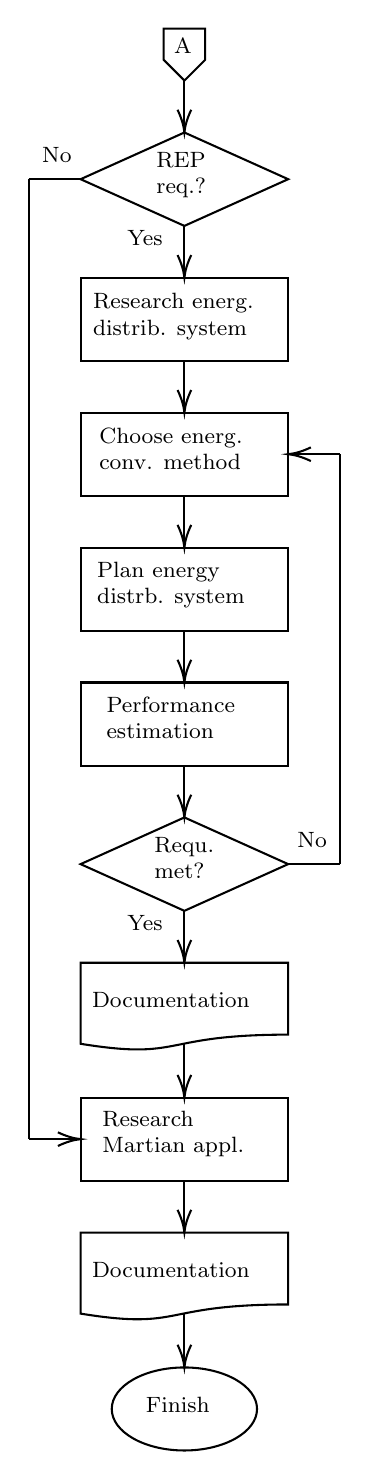
\begin{tikzpicture}[x=0.75pt,y=0.75pt,yscale=-1,xscale=1]
%uncomment if require: \path (0,882); %set diagram left start at 0, and has height of 882

%Pentagon Arrow [id:dp6295335837224703] 
\draw   (365,45) -- (365,60) -- (355,70) -- (345,60) -- (345,45) -- cycle ;

%Shape: Rectangle [id:dp9114846783986272] 
\draw   (305,165) -- (405,165) -- (405,205) -- (305,205) -- cycle ;

%Straight Lines [id:da1841951473424126] 
\draw    (355,70) -- (355,93) ;
\draw [shift={(355,95)}, rotate = 270] [color={rgb, 255:red, 0; green, 0; blue, 0 }  ][line width=0.75]    (10.93,-3.29) .. controls (6.95,-1.4) and (3.31,-0.3) .. (0,0) .. controls (3.31,0.3) and (6.95,1.4) .. (10.93,3.29)   ;
%Shape: Diamond [id:dp3275955259803509] 
\draw   (355,95) -- (405,117.5) -- (355,140) -- (305,117.5) -- cycle ;
%Straight Lines [id:da6311173750553984] 
\draw    (355,140) -- (355,163) ;
\draw [shift={(355,165)}, rotate = 270] [color={rgb, 255:red, 0; green, 0; blue, 0 }  ][line width=0.75]    (10.93,-3.29) .. controls (6.95,-1.4) and (3.31,-0.3) .. (0,0) .. controls (3.31,0.3) and (6.95,1.4) .. (10.93,3.29)   ;

%Shape: Rectangle [id:dp913835377980921] 
\draw   (305,230) -- (405,230) -- (405,270) -- (305,270) -- cycle ;

%Straight Lines [id:da3649991025923325] 
\draw    (355,205) -- (355,228) ;
\draw [shift={(355,230)}, rotate = 270] [color={rgb, 255:red, 0; green, 0; blue, 0 }  ][line width=0.75]    (10.93,-3.29) .. controls (6.95,-1.4) and (3.31,-0.3) .. (0,0) .. controls (3.31,0.3) and (6.95,1.4) .. (10.93,3.29)   ;
%Straight Lines [id:da43992652550284816] 
\draw    (355,270) -- (355,293) ;
\draw [shift={(355,295)}, rotate = 270] [color={rgb, 255:red, 0; green, 0; blue, 0 }  ][line width=0.75]    (10.93,-3.29) .. controls (6.95,-1.4) and (3.31,-0.3) .. (0,0) .. controls (3.31,0.3) and (6.95,1.4) .. (10.93,3.29)   ;
%Shape: Rectangle [id:dp9403171441896898] 
\draw   (305,295) -- (405,295) -- (405,335) -- (305,335) -- cycle ;

%Shape: Rectangle [id:dp553852729933479] 
\draw   (305,360) -- (405,360) -- (405,400) -- (305,400) -- cycle ;
%Straight Lines [id:da1550632508471741] 
\draw    (355,335) -- (355,358) ;
\draw [shift={(355,360)}, rotate = 270] [color={rgb, 255:red, 0; green, 0; blue, 0 }  ][line width=0.75]    (10.93,-3.29) .. controls (6.95,-1.4) and (3.31,-0.3) .. (0,0) .. controls (3.31,0.3) and (6.95,1.4) .. (10.93,3.29)   ;
%Straight Lines [id:da1341632742496266] 
\draw    (355,400) -- (355,423) ;
\draw [shift={(355,425)}, rotate = 270] [color={rgb, 255:red, 0; green, 0; blue, 0 }  ][line width=0.75]    (10.93,-3.29) .. controls (6.95,-1.4) and (3.31,-0.3) .. (0,0) .. controls (3.31,0.3) and (6.95,1.4) .. (10.93,3.29)   ;
%Shape: Diamond [id:dp8080302672223327] 
\draw   (355,425) -- (405,447.5) -- (355,470) -- (305,447.5) -- cycle ;

%Straight Lines [id:da3135121459732009] 
\draw    (407,250) -- (430,250) ;
\draw [shift={(405,250)}, rotate = 0] [color={rgb, 255:red, 0; green, 0; blue, 0 }  ][line width=0.75]    (10.93,-3.29) .. controls (6.95,-1.4) and (3.31,-0.3) .. (0,0) .. controls (3.31,0.3) and (6.95,1.4) .. (10.93,3.29)   ;
%Straight Lines [id:da1661173997317298] 
\draw    (430,250) -- (430,447.5) ;
%Straight Lines [id:da013009727986448727] 
\draw    (430,447.5) -- (405,447.5) ;

%Straight Lines [id:da8133901261188266] 
\draw    (355,470) -- (355,493) ;
\draw [shift={(355,495)}, rotate = 270] [color={rgb, 255:red, 0; green, 0; blue, 0 }  ][line width=0.75]    (10.93,-3.29) .. controls (6.95,-1.4) and (3.31,-0.3) .. (0,0) .. controls (3.31,0.3) and (6.95,1.4) .. (10.93,3.29)   ;

%Flowchart: Document [id:dp6420835715080364] 
\draw   (305,495) -- (405,495) -- (405,529.65) .. controls (342.5,529.65) and (355,542.15) .. (305,534.06) -- cycle ;

%Straight Lines [id:da3287541689868827] 
\draw    (355,534) -- (355,558) ;
\draw [shift={(355,560)}, rotate = 270] [color={rgb, 255:red, 0; green, 0; blue, 0 }  ][line width=0.75]    (10.93,-3.29) .. controls (6.95,-1.4) and (3.31,-0.3) .. (0,0) .. controls (3.31,0.3) and (6.95,1.4) .. (10.93,3.29)   ;

%Shape: Rectangle [id:dp9760404082725573] 
\draw   (305,560) -- (405,560) -- (405,600) -- (305,600) -- cycle ;
%Flowchart: Document [id:dp2517134736579656] 
\draw   (305,625) -- (405,625) -- (405,659.65) .. controls (342.5,659.65) and (355,672.15) .. (305,664.06) -- cycle ;

%Straight Lines [id:da5089558784451147] 
\draw    (355,664) -- (355,688) ;
\draw [shift={(355,690)}, rotate = 270] [color={rgb, 255:red, 0; green, 0; blue, 0 }  ][line width=0.75]    (10.93,-3.29) .. controls (6.95,-1.4) and (3.31,-0.3) .. (0,0) .. controls (3.31,0.3) and (6.95,1.4) .. (10.93,3.29)   ;

%Straight Lines [id:da19223774212748634] 
\draw    (355,600) -- (355,623) ;
\draw [shift={(355,625)}, rotate = 270] [color={rgb, 255:red, 0; green, 0; blue, 0 }  ][line width=0.75]    (10.93,-3.29) .. controls (6.95,-1.4) and (3.31,-0.3) .. (0,0) .. controls (3.31,0.3) and (6.95,1.4) .. (10.93,3.29)   ;
%Straight Lines [id:da9396270466808674] 
\draw    (280,580) -- (303,580) ;
\draw [shift={(305,580)}, rotate = 180] [color={rgb, 255:red, 0; green, 0; blue, 0 }  ][line width=0.75]    (10.93,-3.29) .. controls (6.95,-1.4) and (3.31,-0.3) .. (0,0) .. controls (3.31,0.3) and (6.95,1.4) .. (10.93,3.29)   ;
%Straight Lines [id:da020572157364605825] 
\draw    (280,117.5) -- (305,117.5) ;

%Straight Lines [id:da680181864059918] 
\draw    (280,117.5) -- (280,580) ;
%Shape: Ellipse [id:dp16223416818247482] 
\draw   (320,710) .. controls (320,698.95) and (335.67,690) .. (355,690) .. controls (374.33,690) and (390,698.95) .. (390,710) .. controls (390,721.05) and (374.33,730) .. (355,730) .. controls (335.67,730) and (320,721.05) .. (320,710) -- cycle ;

% Text Node
\draw (348.5,48) node [anchor=north west][inner sep=0.75pt]  [font=\footnotesize] [align=left] {A};
% Text Node
\draw (309.5,171) node [anchor=north west][inner sep=0.75pt]  [font=\footnotesize] [align=left] {Research energ.\\distrib. system};
% Text Node
\draw (340,103) node [anchor=north west][inner sep=0.75pt]  [font=\footnotesize] [align=left] {REP\\req.?};
% Text Node
\draw (326,140.5) node [anchor=north west][inner sep=0.75pt]  [font=\footnotesize] [align=left] {Yes};
% Text Node
\draw (312.5,236) node [anchor=north west][inner sep=0.75pt]  [font=\footnotesize] [align=left] {Choose energ.\\conv. method};
% Text Node
\draw (311.5,300.5) node [anchor=north west][inner sep=0.75pt]  [font=\footnotesize] [align=left] {Plan energy\\distrb. system};
% Text Node
\draw (316,365.5) node [anchor=north west][inner sep=0.75pt]  [font=\footnotesize] [align=left] {Performance\\estimation};
% Text Node
\draw (339,433) node [anchor=north west][inner sep=0.75pt]  [font=\footnotesize] [align=left] {Requ.\\met?};
% Text Node
\draw (408,430.5) node [anchor=north west][inner sep=0.75pt]  [font=\footnotesize] [align=left] {No};
% Text Node
\draw (326,470.5) node [anchor=north west][inner sep=0.75pt]  [font=\footnotesize] [align=left] {Yes};
% Text Node
\draw (309,508) node [anchor=north west][inner sep=0.75pt]  [font=\footnotesize] [align=left] {Documentation};
% Text Node
\draw (314,565) node [anchor=north west][inner sep=0.75pt]  [font=\footnotesize] [align=left] {Research\\Martian appl.};
% Text Node
\draw (309,638) node [anchor=north west][inner sep=0.75pt]  [font=\footnotesize] [align=left] {Documentation};
% Text Node
\draw (285,100.5) node [anchor=north west][inner sep=0.75pt]  [font=\footnotesize] [align=left] {No};
% Text Node
\draw (335,703) node [anchor=north west][inner sep=0.75pt]  [font=\footnotesize] [align=left] {Finish};


\end{tikzpicture}

	\caption{Part two of the flowchart of this thesis. It illustartes which steps were taken in order to achieve the deliverables.}
	\label{fig:tikz_flowchart_2}
\end{figure}

\subsection{Thesis Structure}
The first part of this thesis contains the \textbf{Methodology} in which the mathematical fundamentals for the system design and the performance estimations of the self-sufficient energy distribution and the voice communication system are explained. This is followed by the \textbf{Results}, presenting the system design and the results of the performance estimations. Finally, the \textbf{Conclusion and critical reflecion} summarizes and interprets the results and provides a critical reflection of this thesis. The appendices contain information about the OeWF and the Serenity spacesuit simulator, mathematical basics and the developed \MATLAB simulation for the performance estimation of the self-sufficient energy distribution system.

